
According to the work of \citeauthor{barroso2007case}~\cite{barroso2007case}, servers operate most of the time at between 10 and 50 percent of their maximum utilization levels.
Moreover, as shown in Figure~\ref{fig:soa_energy_efficiency} with 50\% of the servers' capacity, the server operates only with 75\% of its maximum power.
In other words, it will cost us only 25\% of the energy to operate the extra 50\% of the servers' capacity.

\begin{figure}[!h]
    \centering
    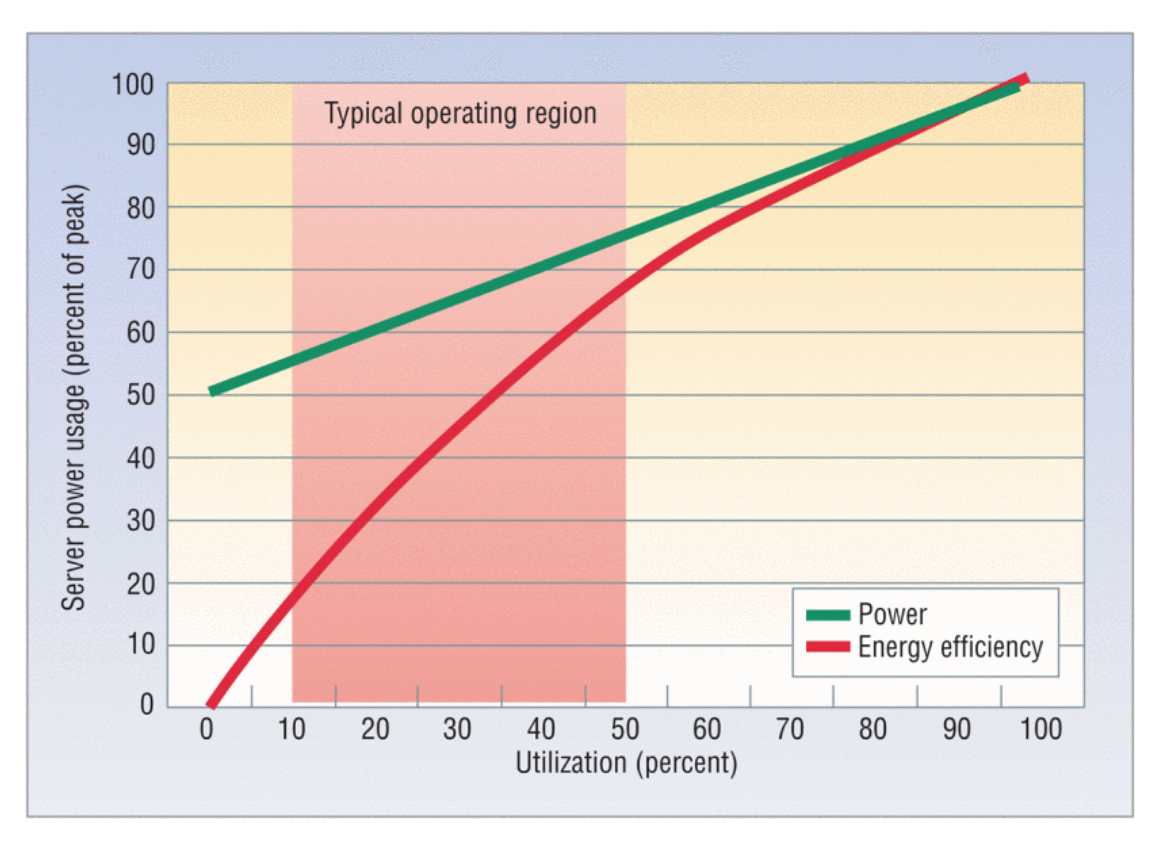
\includegraphics[width=.7\linewidth,keepaspectratio]{chapters/soa_energy_efficiency}
    \caption{Power efficiency Vs. power consumption~\cite{barroso2007case}}
    \label{fig:soa_energy_efficiency}
\end{figure}

To confirm if this hypothesis still holds, we run the following experiment.
First, we provision a machine with minimal services, then created a process that stresses one core by doing some mathematical operations, and each second we introduced a copy of this process.
After a while, we removed these copies one by one.
The source code of the experiment can be found in the following GitHub repository.\link{https://github.com/chakib-belgaid/lazy-green-code-test}
Figure~\ref{fig:power_evolution_greenfaas} reports on the machine power consumption during this experiment.
As one can notice, the introduction of the first copies had a greater cost than the other ones, despite not sharing the same core.
And the more we approach the peak of power, the less significance the introduction of a new process has on power consumption to be almost zero after the $9^{th}$ copy.

\begin{figure}[!h]
    \centering
    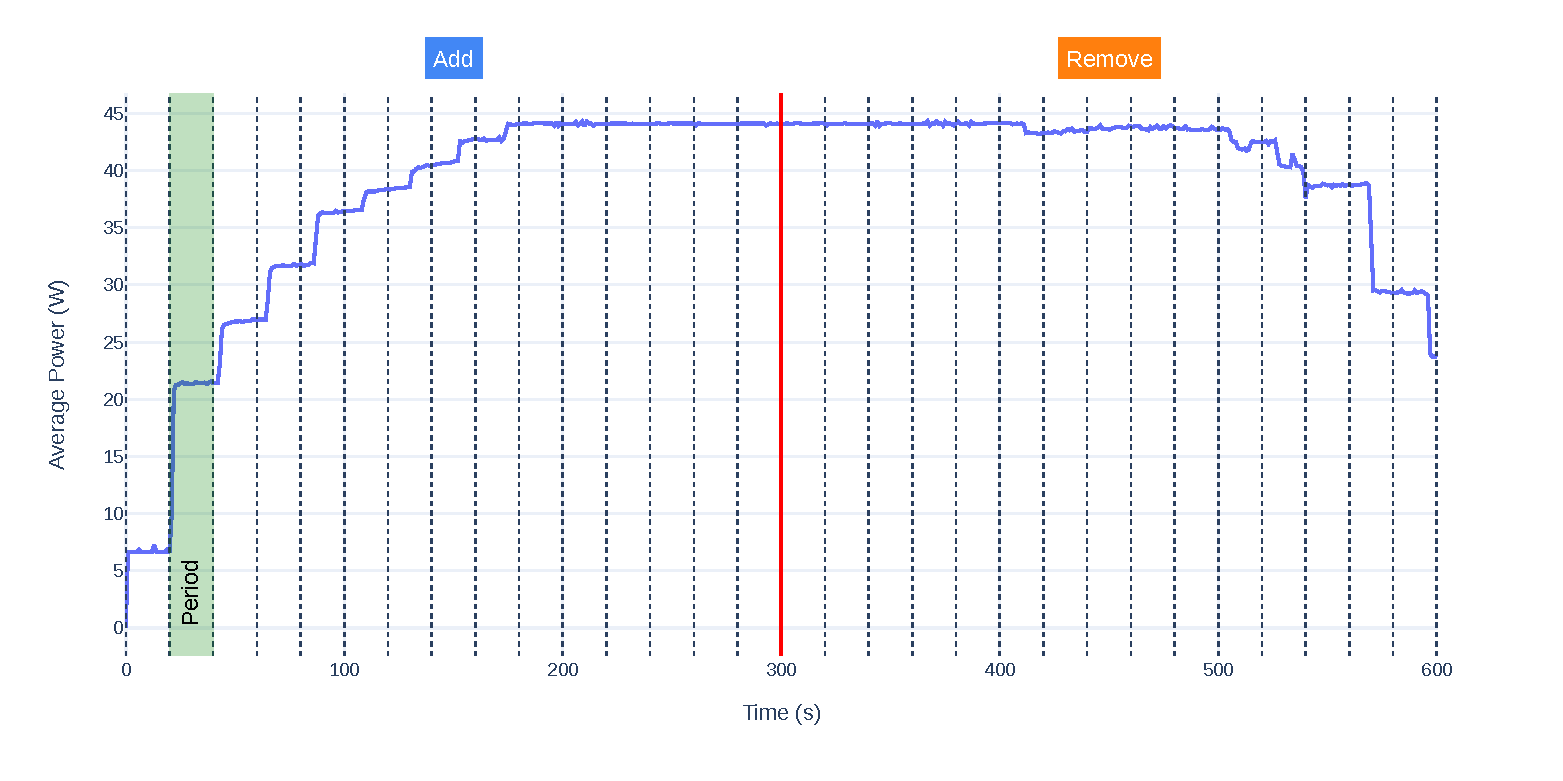
\includegraphics[width=\linewidth]{chapters/power_evolution_greenfaas}
    \caption{Evolution of CPU power}
    \label{fig:power_evolution_greenfaas}
\end{figure}

One should note that this experiment was conducted on a machine with the following configuration: Intel(R) Core(TM) i7-3740QM CPU @ 2.70GHz, with 4 physical cores and 4 hyper threads, 16GB RAM, and 687GB HDD.
As for the operating system, we used Ubuntu 20.04.2 LTS.

Therefore, with the introduction of the $8^{th}$ copy, we have already saturated the machine capacity, and the introduction of the $9^{th}$ copy had no impact on the power consumption.

To push this experiment further, we created a stress tool to fix the number of cores and \% usage of each core to simulate a production context.
We then run a benchmark (graph coloration algorithm)\link{https://github.com/chakib-belgaid/lazy-green-code-test/tree/master/exp01} using multiple configurations.
Figure~\ref{fig:green_faas_duration} displays the overall performance of the benchmark.
As one can see, the execution time remained the same when the context was using 3 cores at any saturation level, because we have 4 physical CPU cores, therefore each process was running a different core (3 cores were used by the context and the other one was used by the benchmark).
However, behavior changes when the context consumes more than 3 cores.
CPU saturation tends to have a greater impact on the performance of the benchmark.
When the benchmark was using a hyper-thread of the same core as one of the context workers, it took almost double the time to finish the same job.
As when we saturated only 50\% of the CPU capacity, this increase did not happen until the context used 7 cores and, in the worst-case scenario (10 extra processes), it took only 75 seconds to finish the job.

\begin{figure}[!h]
    \centering
    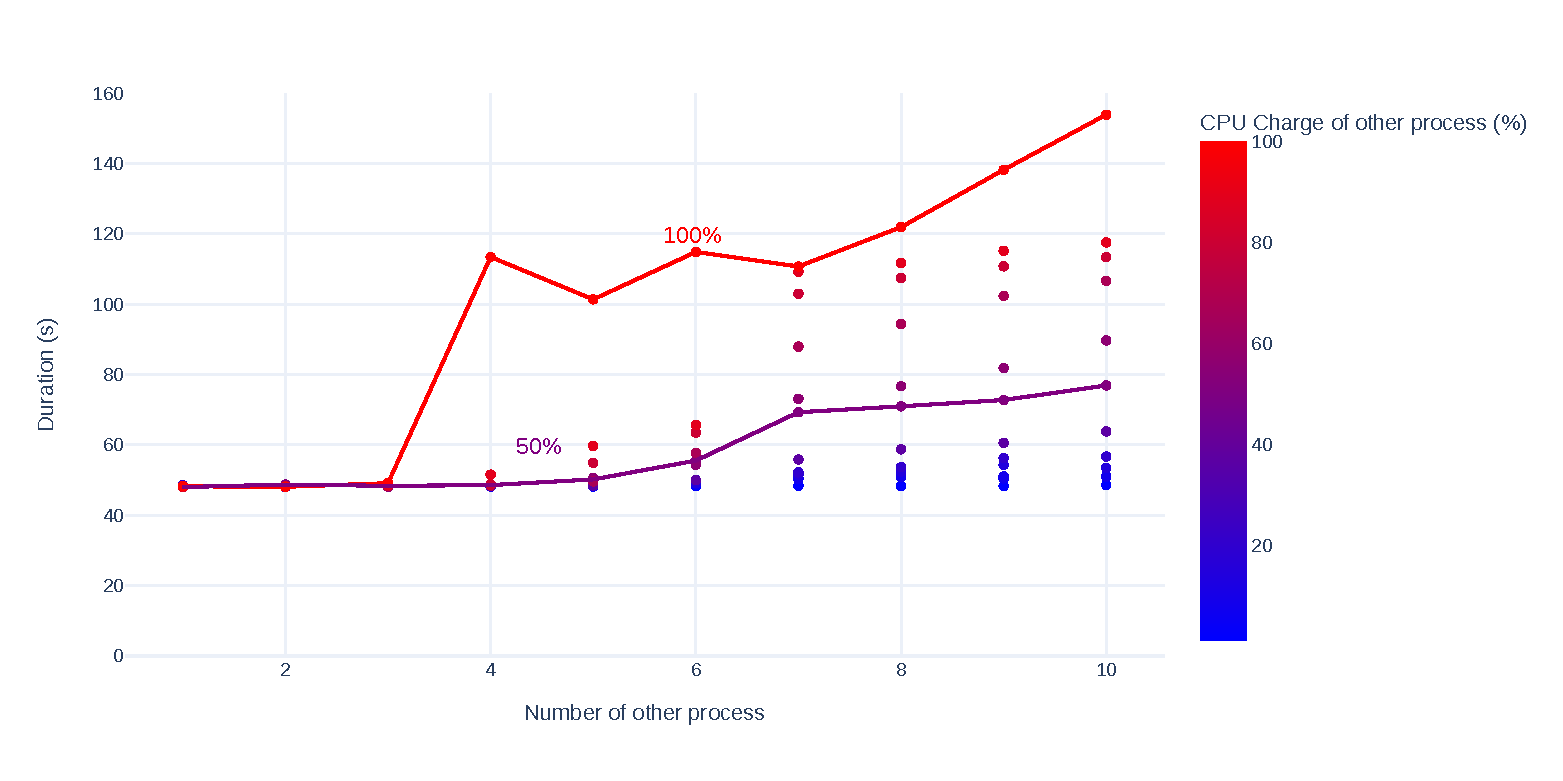
\includegraphics[width=\linewidth]{chapters/green_faas_duration}
    \caption{Evolution of CPU behavior during multiple contexts }
    \label{fig:green_faas_duration}
\end{figure}

On the other hand, as we can see in Figure~\ref{fig:green_faas_power}, the average power behavior of the system had different behavior.
With the 100\% saturation scenario, the power consumption hit its peak as soon as we hit the 4 core usage 3 from the context and 1 from the benchmark), and it kept fluctuating until the $8^{th}$ core saturation, after that, it was in a constant decrease.
This was because the processes were competing with each other for cache usage, which led to a significant number of cache misses that slowed down the CPU frequency and led to a decrease in power consumption.

\begin{figure}[!h]
    \centering
    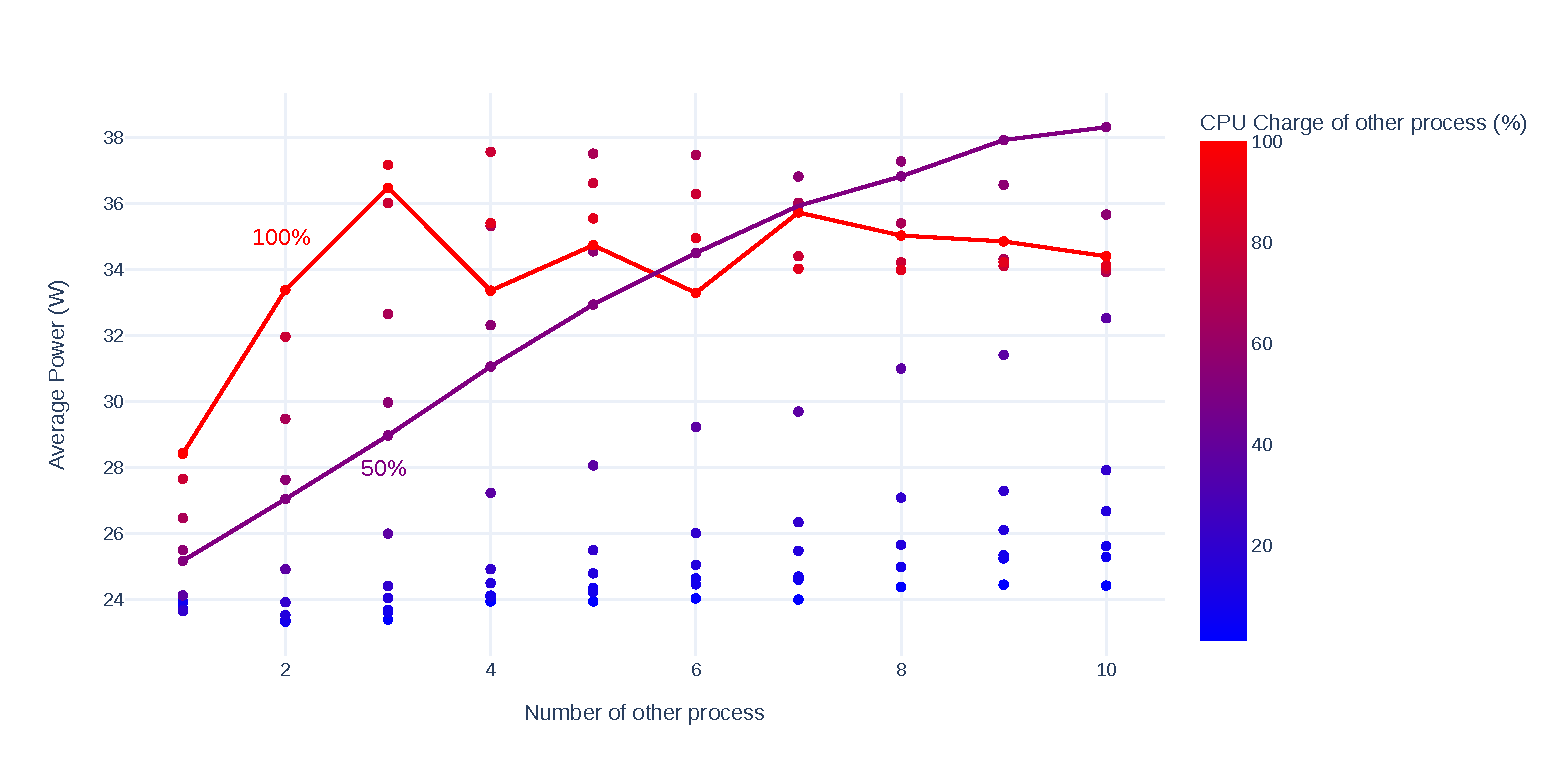
\includegraphics[width=\linewidth]{chapters/green_faas_power}
    \caption{Evolution of CPU behavior during multiple contexts }
    \label{fig:green_faas_power}
\end{figure}


However, when we used 50\% of the CPU capacity, the power kept increasing by adding the number of extra processes.
As for the scenarios where we used more than 50\% of the CPU capacity, the power consumption kept increasing until it hit its peak then it start to decrease; this number of processes needed to reach the peak varies according to the saturation level.

When we try to measure the energy consumption of this experiment, we find that the scenario where we used 100\% of the energy consumption was the worst case by far, and it kept increasing whenever we increase the number of core usage.
Figure~\ref{fig:green_faas_energy} present the energy consumption of the system during the experiment.

\begin{figure}[!h]
    \centering
    \caption{Evolution of CPU behavior during multiple contexts }
    \label{fig:green_faas_energy}
    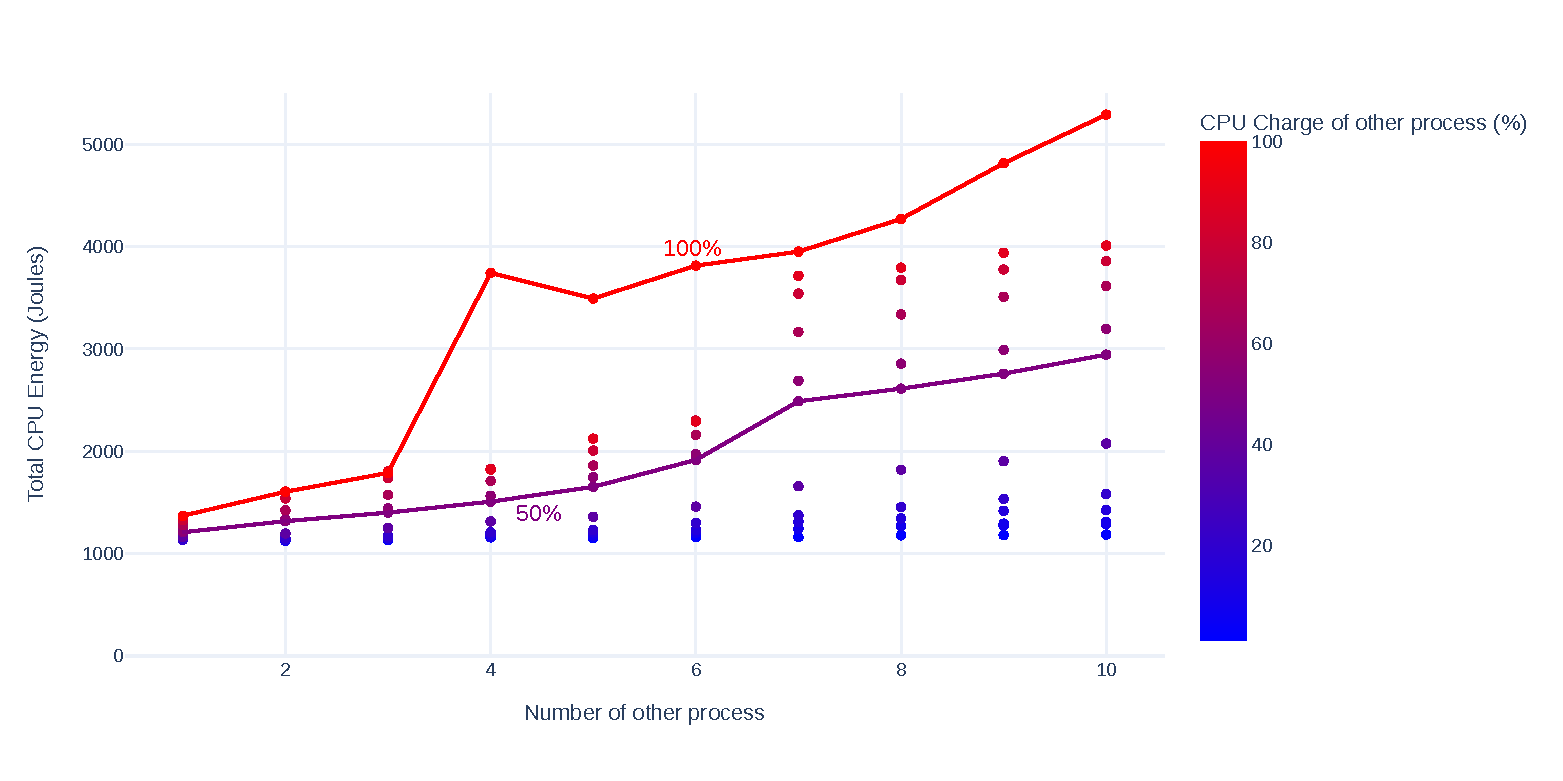
\includegraphics[width=\linewidth]{chapters/green_faas_energy}
\end{figure}

However, if we calculate the energy impact of the benchmark which we define as:
\begin{equation}
    Impact_{Benchmark} =E_{Benchmark} - E_{Before}
\end{equation}
and can be approximated by:
\begin{equation}
    Impact_{Benchmark} =E_{Benchmark} - P_{Before} * T_{Benchmark}
\end{equation}
where $Impact_{Benchmark}$ is the energy impact of the benchmark, $E_{Benchmark}$ is the energy of the system when the benchmark is running, $E_{Before}$ is the energy of the system before the benchmark is running, $P_{Before}$ is the power of the system before the benchmark is running, and $T_{Benchmark}$ is the time of the benchmark execution.

One can notice that the energy impact of our benchmark did not have the same behavior as the system's energy consumption.
Sometimes, introducing the benchmark had a \emph{negative} impact on the system's energy consumption, which made it even greener.
This is because it reduces power consumption.
This is shown in Figure~\ref{fig:green_faas_impact}.

\begin{figure}[!t]
    \centering
    \caption{Evolution of CPU behavior during multiple contexts }
    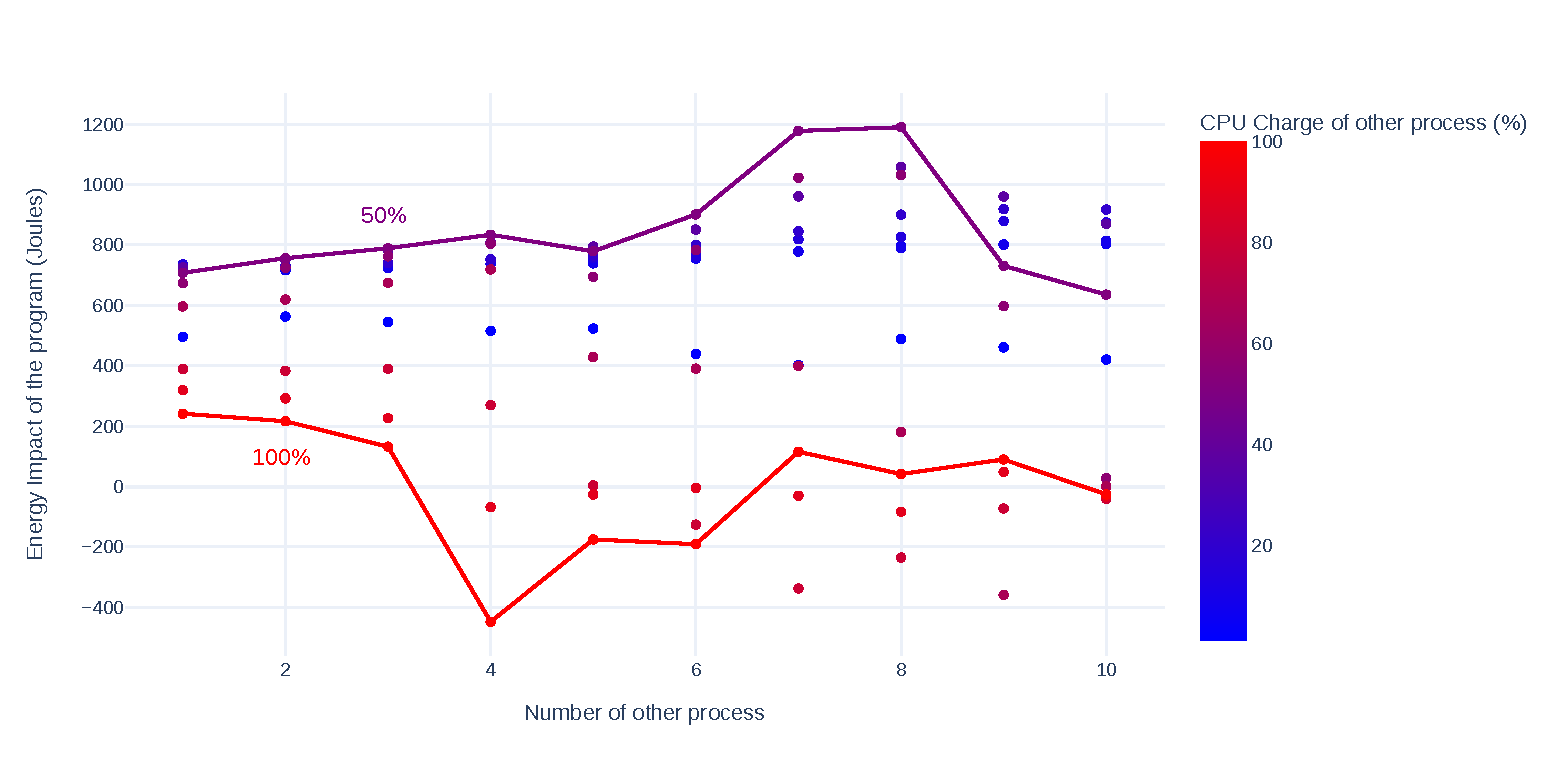
\includegraphics[width=\linewidth]{chapters/green_faas_impact}\
    \label{fig:green_faas_impact}
\end{figure}

We are aware that during this analysis, we have not considered the execution time of the context, and it will be affected by the benchmark---mainly, it will increase when we use more cores and/or higher CPU saturation.
However, this action was motivated by the fact that most of the cloud software is web services, as we have seen in Chapter~\ref{chapter:porgramming_langauges} where the execution time is not bounded, and each service can run for an unlimited amount of time.

\paragraph*{Synthesis}
This experiment shows that the context can have a significant impact on the energy consumption of the system, and sometimes measuring only the energy consumption of an application does not represent the real impact of this application on the energy consumption of the whole system, especially when we are dealing with timeless Softwares aka services.
In the future, we tend to extend this experiment with more data, such as the energy consumption of the application itself instead of the whole system using \cite{fieni2020smartwatts} and comparing the strategies that were mentioned in this thesis using multiple contexts instead of just a minimal version of the operating system.
